% supplementary.tex — supplementary material for manuscript.tex. Compile: latexmk -pdf supplementary.tex
% Every number is taken from a repository file named in the table captions.
\documentclass[11pt]{article}
\usepackage[utf8]{inputenc}
\usepackage[T1]{fontenc}
\usepackage{lmodern}
\usepackage[margin=2.5cm]{geometry}
\usepackage{amsmath,amssymb}
\usepackage{graphicx}
\usepackage{booktabs}
\usepackage{tabularx}
\usepackage[hidelinks]{hyperref}
\usepackage{microtype}
\graphicspath{{figures/}}
\renewcommand{\thetable}{S\arabic{table}}
\renewcommand{\thefigure}{S\arabic{figure}}
\renewcommand{\thesection}{S\arabic{section}}

\title{Supplementary material for ``Deadlocks of Learned Navigation Policies Behind a Control-Barrier-Function Safety Filter: Mechanisms and Planning-Based Recovery''}
\author{Pouya Bathaei Pourmand}
\date{17 November 2026}

\begin{document}
\maketitle

\noindent Contents: S1 configuration; S2 recovery-layer parameters; S3 pre-registration record; S4 additional round-4 results; S5 timeout analysis; S6 statistical procedures; S7 additional analyses of the first round; S8 reproduction. Code, data and the full protocols are at \url{https://github.com/pouyapd/SafeNav-RL}.

%=====================================================================
\section{Simulation, filter and training configuration}
%=====================================================================
\begin{table}[htbp]
\centering\small
\caption{Configuration of all experiments (\texttt{configs/default\_config.yaml}; stage values are the requested ones).}
\begin{tabularx}{\linewidth}{@{}lX@{}}
\toprule
Item & Value \\
\midrule
Workspace, time step & $[0,10]^2$\,m; $\Delta t=0.1$\,s; forward-Euler unicycle, $v\in[0,1]$\,m/s, $\omega\in[-1,1]$\,rad/s \\
Robot, goal & disc of radius 0.3\,m; success within 0.5\,m of the goal \\
Observation & noisy position ($\sigma=0.02$\,m), $\sin\theta,\cos\theta$, goal distance and bearing, proximity (risk) feature, 16 range beams up to 3\,m ($\sigma=0.02$\,m) \\
Filter & one-step DT-CBF on the speed; safety margin 0.3\,m from obstacle surfaces, 0.1\,m from walls; $\gamma=0.5\,\mathrm{s}^{-1}$ \\
Reward & step $-0.01$; distance shaping $\alpha=1$; risk penalty $\beta=0.5$ (risk falls from 1 at a surface to 0 at 0.8\,m); goal $+10$; collision $-5$ \\
Curriculum (requested) & beginner 2--4 obstacles, goal 3--5\,m, 200 steps; intermediate 4--8, 5--8\,m, 300 steps; expert 8--15, 5--12\,m, 400 steps; advance at 70\,\% success over 100 episodes. Obstacles that do not fit are skipped: 8--12 were placed in the 100 expert test scenarios \\
PPO & $10^6$ steps; rollout 2048; 10 epochs; batch 64; $\gamma=0.99$; GAE $\lambda=0.95$; clip 0.2; value coefficient 0.5; entropy 0.01; gradient norm 0.5; learning rate $3\cdot10^{-4}$, linear decay \\
Networks & separate actor and critic, $256\times256$, tanh; Gaussian policy, initial $\log\sigma=-0.5$, clamped to $[-3,1]$ \\
Checkpoint selection & best validation success on 60 episodes (20 per stage), validation seeds disjoint from all test seeds \\
Training arms of E1a/E4 & as above but 300k steps; E1a adds the correction penalty ($\alpha=1$); E4 uses a Beta policy or $\beta=0$ \\
\bottomrule
\end{tabularx}
\end{table}

%=====================================================================
\section{Recovery-layer parameters}
%=====================================================================
\begin{table}[htbp]
\centering\small
\caption{Parameters of the recovery layer (\texttt{safenav/recovery/controller.py}, \texttt{planner.py}). All were fixed before the round-3 pilot and not tuned; round 4 used the same values.}
\begin{tabularx}{\linewidth}{@{}lX@{}}
\toprule
Parameter & Value \\
\midrule
Cost-to-go & shortest-path length to the goal region through the safe set; 8-connected Dijkstra on a 5\,cm grid; built once per episode \\
Manoeuvre library & 65 sequences of 40 steps: turn in place at $\pm1$\,rad/s for $k\in\{0,4,8,12,16,24,31\}$ steps, then $v=1$\,m/s with $\omega\in\{0,\pm0.5,\pm1\}$\,rad/s \\
Prediction & every sequence rolled out through the exact unicycle model with the filter \\
Trigger (B, C) & net displacement below 0.15\,m over the last 30 steps \\
C: replanning, exit & replan every 5 steps; exit when the cost-to-go has fallen by 1.0\,m, when the best sequence gains less than 0.1\,m, or after 100 steps \\
A: trigger, commitment & filter speed limit below 0.1\,m/s or commanded speed at most 0.05\,m/s; plan used if it beats holding the command by 0.5\,m; 10 committed steps \\
B: behaviour & turn to the tangent of the nearest barrier (gain 2.0, tolerance 0.1\,rad), then 30 steps of tangent following \\
Planner only (round 4) & the planner of C from the first step, replanned every 5 steps \\
Path followers (round 4) & pure pursuit (look-ahead 0.5\,m, turn gain 2.0, $v_{\max}=1$\,m/s) along the steepest descent of the cost-to-go; the inflated variant plans with 0.2\,m extra clearance \\
Information models (round 4) & position noise $\mathcal N(0,0.05\,\mathrm m)$ per axis and heading noise $\mathcal N(0,0.05\,\mathrm{rad})$, fresh each step; map error: centres $+\mathcal N(0,0.1\,\mathrm m)$, radii $\times\,\mathcal U(0.85,1.15)$, each obstacle missing with probability 0.1, fixed per episode; sensed map: an obstacle enters the map once one of 16 range beams (3\,m) hits it \\
\bottomrule
\end{tabularx}
\end{table}

%=====================================================================
\section{Pre-registration record}
%=====================================================================
Each hypothesis-testing evaluation had its protocol, decision rules and analysis code committed and pushed before it was run. Exploratory analyses are labelled as such in the manuscript.

\begin{table}[htbp]
\centering\small
\caption{Protocols and the commits that fixed them before the runs (repository history).}
\begin{tabularx}{\linewidth}{@{}lXl@{}}
\toprule
Round & Content & Protocol commit \\
\midrule
1 & 500 fresh expert scenarios: replication, heading escape, final checkpoints (\texttt{research/experiments/lightweight/}) & \texttt{9ced888} \\
2 & E1a correction penalty (\texttt{research/experiments/e1a/}) & \texttt{d65e576} \\
2 & E3 corrected generator, E4 self-stop causes, DWA (\texttt{research/experiments/round2/}) & \texttt{cbbe766}, \texttt{3aed35e}; DWA margin note \texttt{8702fb7} \\
3 & recovery methods A, B, C, C with a straight-line cost (\texttt{research/experiments/round3/}) & \texttt{c1abd93}; amendment \texttt{5d2838d} \\
4 & latency (P), robustness (R), fairness (F), timeouts (T) (\texttt{research/experiments/round4/}) & \texttt{c0629f7}; amendment \texttt{f0194a1} \\
\bottomrule
\end{tabularx}
\end{table}

\noindent Round-4 amendment 1, made after the pilots and before every confirmatory run, added an exploratory path-follower variant with an inflated margin and a supplementary recovery-success threshold; no method, endpoint, scenario set or hypothesis was changed. Independent audits recomputed the earlier rounds with separate code: round 2 by \texttt{research/experiments/round3/audit\_round2.py} (223 checks) and round 3 by \texttt{research/experiments/round4/audit\_round3.py} (68 checks, 0 failed; 776 episodes without a run record replayed identically).

%=====================================================================
\section{Additional round-4 results}
%=====================================================================
\begin{table}[htbp]
\centering\small
\caption{All methods on the same 200 expert scenarios (round 4, seeds from $4.4\cdot10^6$). Rates in \%; learned methods ``with / without'' filter in training (1{,}000 episodes each), map-based methods 200 episodes. Source: \texttt{research/experiments/round4/results/summary.json}.}
\resizebox{\linewidth}{!}{%
\begin{tabular}{@{}lcccccc@{}}
\toprule
Method & Success & Collision & Deadlock & Filter-blocked & Moving timeout & Planner calls / ep. \\
\midrule
policy, no filter & 54.0 / 94.1 & 9.1 / 1.0 & 35.7 / 4.9 & 0 / 0 & 1.2 / 0.0 & 0 \\
policy + filter (baseline) & 43.0 / 49.1 & 0 & 54.9 / 50.8 & 19.7 / 45.2 & 2.1 / 0.1 & 0 \\
A & 90.0 / 94.9 & 0 & 5.4 / 1.6 & 3.2 / 1.6 & 4.6 / 3.5 & 22.9 / 12.3 \\
C & 86.3 / 85.2 & 0 & 0.2 / 0.3 & 0.1 / 0.3 & 13.5 / 14.5 & 11.1 / 9.8 \\
C, position noise & 84.5 / 84.7 & 0 & 0.1 / 0.2 & 0.1 / 0.1 & 15.4 / 15.1 & 13.2 / 11.6 \\
C, map error & 71.5 / 71.6 & 0 & 18.4 / 21.3 & 17.7 / 20.9 & 10.1 / 7.1 & 16.1 / 15.4 \\
C, sensed map & 86.6 / 85.2 & 0 & 0.1 / 0.5 & 0.1 / 0.5 & 13.3 / 14.3 & 11.3 / 9.9 \\
planner only & 95.0 & 0 & 3.0 & 2.5 & 2.0 & 35.1 \\
shortest-path follower & 11.0 & 0 & 89.0 & 89.0 & 0.0 & -- \\
path follower, +0.2\,m (exploratory) & 64.5 & 0 & 35.5 & 35.5 & 0.0 & -- \\
\bottomrule
\end{tabular}}
\end{table}

\begin{table}[htbp]
\centering\small
\caption{Imperfect versus exact information: C$_k$ $-$ C on the same scenarios (points, 95\,\% paired hierarchical bootstrap intervals; unadjusted secondary contrasts). Source: as Table S4.}
\begin{tabular}{@{}llccc@{}}
\toprule
Condition & Agents & $\Delta$ deadlock & $\Delta$ success & $\Delta$ moving timeouts \\
\midrule
position noise & with & $-0.1$ [$-0.6$, 0.4] & $-1.8$ [$-4.1$, 0.2] & $+1.9$ [$-0.1$, 4.2] \\
 & w/o & $-0.1$ [$-0.9$, 0.7] & $-0.5$ [$-2.1$, 0.8] & $+0.6$ [$-1.1$, 2.6] \\
map error & with & $+18.2$ [13.7, 22.8] & $-14.8$ [$-18.9$, $-10.8$] & $-3.4$ [$-7.4$, 0.2] \\
 & w/o & $+21.0$ [15.8, 26.5] & $-13.6$ [$-18.2$, $-9.2$] & $-7.4$ [$-12.4$, $-2.4$] \\
sensed map & with & $-0.1$ [$-0.6$, 0.0] & $+0.3$ [$-0.9$, 1.5] & $-0.2$ [$-1.3$, 0.9] \\
 & w/o & $+0.2$ [0.0, 0.8] & $+0.0$ [$-1.0$, 1.0] & $-0.2$ [$-1.4$, 0.9] \\
\bottomrule
\end{tabular}
\end{table}

\paragraph{Recovery activity.} Recovery success (an activation that lowers the cost-to-go by at least 1\,m at the true position) was 0.87 / 0.86 for C, 0.34 / 0.36 with position noise (0.81 / 0.78 at the supplementary 0.8\,m threshold of the amendment: the exit test fires on the noisy estimate), 0.31 / 0.21 with map error and 0.86 / 0.84 with the sensed map, which rebuilt its map about 5.9 times per episode and knew about 7.2 obstacles at the end.

\begin{table}[htbp]
\centering\small
\caption{Latency test (Part P): 4{,}000 episodes (methods A and C, each with both planners, on 100 new expert scenarios), one laptop (Intel Core i7-1255U, Windows 11, Python 3.12.7, NumPy 2.4.1), normal priority, mains power, the user's other applications running (about 33\,\% system load). Not a real-time guarantee. Source: \texttt{research/experiments/round4/results/summary.json}.}
\begin{tabular}{@{}lcc@{}}
\toprule
Planner call (38{,}041 paired calls) & Reference & Fast (identical plans) \\
\midrule
wall p50 / p90 / p95 / p99 / max (ms) & 8.1 / 18.4 / 26.4 / 45.7 / 480.6 & 4.5 / 10.2 / 15.0 / 25.0 / 224.9 \\
CPU p50 / p99 / max (ms) & 8.0 / 31.2 / 54.4 & 4.4 / 18.7 / 40.6 \\
calls $\ge$ 100\,ms (all pre-empted) & 17 & 9 \\
control steps $\ge$ 100\,ms (of 419{,}777) & 57 & 12 \\
per-episode longest step, p99 (ms) & 123.0 & 79.7 \\
\bottomrule
\end{tabular}
\end{table}

\begin{figure}[htbp]
\centering
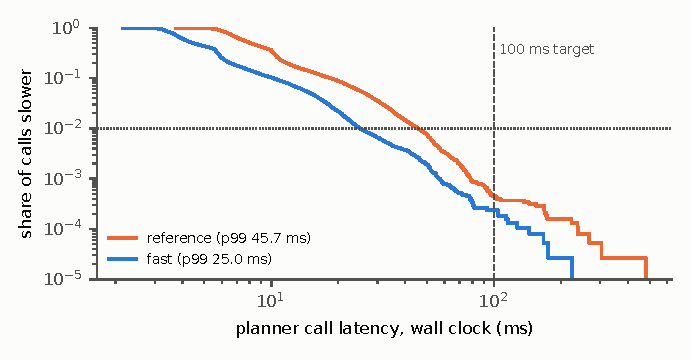
\includegraphics[width=0.7\linewidth]{r4_latency.pdf}
\caption{Share of planner calls slower than a given wall-clock latency (log--log), both planners, Part P. Source: \texttt{research/experiments/round4/results/latency/calls.csv}.}
\end{figure}

\noindent Profiling (\texttt{research/experiments/round4/profile/}): in the reference planner, the barrier evaluation, called twice per rollout step, took 45--60\,\% of the time, dominated by the per-call overhead of small NumPy operations. The fast planner reduces barrier evaluations per call from 5{,}325 to 1{,}674 on average and the CPU time per call to 0.58 of the reference, with bit-identical plans in 4{,}000 of 4{,}000 recorded calls.

%=====================================================================
\section{Timeout analysis (exploratory)}
%=====================================================================
\begin{table}[htbp]
\centering\small
\caption{Decomposition of the 700 moving timeouts of C in round 3 (all reproduced by replay; medians unless stated). Source: \texttt{research/experiments/round4/timeouts/summary.json}.}
\begin{tabular}{@{}lc@{}}
\toprule
Quantity & Value \\
\midrule
first trigger (step) & 108 \\
steps inside 30-step trigger windows & 90 \\
activations & 3 \\
recovery steps (turning in place / driving) & 138 (70 / 66) \\
policy steps & 262 \\
steps in which the filter lowered the commanded speed & 66\,\% \\
executed / commanded speed & 0.32 \\
mean executed speed (mean over episodes) & 0.22\,m/s \\
start--goal geodesic / progress / remaining (m) & 8.6 / 4.3 / 4.5 \\
episodes with more than 2\,m remaining & 86\,\% \\
episodes in which the policy undid more than 1\,m of progress & 19\,\% \\
\bottomrule
\end{tabular}
\end{table}

\begin{figure}[htbp]
\centering
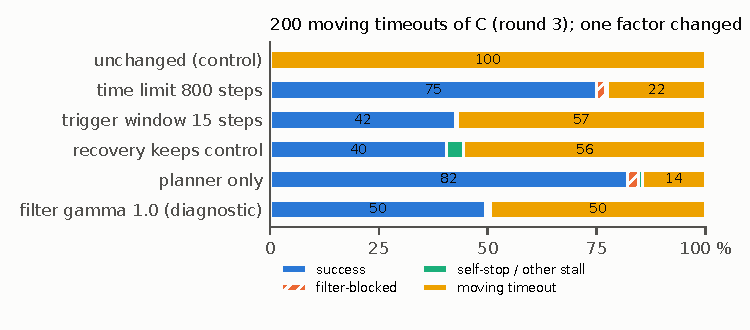
\includegraphics[width=0.75\linewidth]{r4_timeouts.pdf}
\caption{200 sampled moving timeouts of C (round 3) replayed with one factor changed at a time; no collisions in any variant. The sample was selected on the outcome, so the bars show how many of these failures a change rescues, not its effect on all episodes. Filter $\gamma=1.0$ is a diagnostic of conservativeness only. Source: \texttt{research/experiments/round4/timeouts/counterfactuals.csv}.}
\end{figure}

%=====================================================================
\section{Statistical procedures}
%=====================================================================
\begin{itemize}
  \item \textbf{Unit of replication.} The training seed for learned agents (five per arm); scenarios are a second, crossed source of variation.
  \item \textbf{Intervals for differences.} Paired hierarchical bootstrap with 10{,}000 replicates: scenarios are resampled jointly for both conditions; seeds are resampled within each condition, or jointly when the same agents run under both conditions (rounds 3 and 4). Two-sided bootstrap $p$-values.
  \item \textbf{Multiplicity.} Holm adjustment within each pre-registered primary family: 2 tests (E1a), 2 (E4), 4 (round 3), 24 (round 4). Secondary and exploratory contrasts are unadjusted and labelled.
  \item \textbf{Seed level.} Per-seed rates, paired $t$-test over seeds, $d_z$ and Hedges' $g_{av}$ are reported in the experiment directories next to every bootstrap interval.
  \item \textbf{Deterministic baselines.} Wilson intervals over episodes.
  \item \textbf{Latency.} Empirical percentiles over all calls or steps; the fast/reference CPU ratio uses a bootstrap over episodes.
  \item \textbf{Independent recomputation.} Primary contrasts of rounds 2 and 3 were recomputed with separate code and a different bootstrap seed (\nolinkurl{research/experiments/tools/verify_primary.py}; \nolinkurl{research/experiments/round4/audit_round3.py}). Round-4 numbers quoted in the manuscript are checked against the saved results by \nolinkurl{research/scripts/verify_manuscript_round4.py}.
\end{itemize}

%=====================================================================
\section{Additional analyses of the first round}
%=====================================================================
\paragraph{Sources of uncertainty.} The decomposition of expert success shows how much the test scenario matters. Depending on the condition, the scenario term accounts for 25--86\,\% of the sum of squares, against under 2\,\% for the seed term. Seed-only intervals such as those in Table~1 of the main text therefore describe reproducibility of training on these 100 scenarios; they understate the uncertainty about the scenario distribution. An approximate fit of interval width to the number of seeds and scenarios suggests that about 10 seeds and 1{,}000 scenarios per stage would give half-widths near 4--5 points for differences of this kind. Beyond about 1{,}000 scenarios, more seeds help more than more scenarios.

\paragraph{Checkpoint selection.} The final checkpoints of the filter-trained runs have more self-stops than the selected checkpoints: $+11.7$ points [3.0, 20.8]. They have fewer filter-blocked stalls ($-7.0$ [$-13.0$, $-1.5$]) and lower success ($-4.8$ [$-8.8$, $-1.2$]). The increase comes from the three seeds whose selected checkpoint was from early in training (0.1--0.3M steps). Self-stops in these seeds rose from 139, 51 and 105 to 205, 174 and 206. In the seed whose best checkpoint is its final one, the results are identical. Longer training with the filter therefore strengthens the self-stopping behaviour rather than removing it.

%=====================================================================
\section{Reproduction}
%=====================================================================
Software: Python 3.12, PyTorch 2.10 (CPU), NumPy 2.4, Gymnasium 1.2; \texttt{pip install -e ".[dev]"}. Every evaluation is seeded and resumable; analysis scripts read only stored outputs. Main commands (full list: \texttt{paper\_draft/reproducibility\_checklist.md}):
\begin{verbatim}
python -m pytest -q                                   # 166 tests
python research/experiments/round3/run_recovery.py --tag main ...   # round 3
python research/experiments/round3/analyze_round3.py --tag main
bash research/experiments/round4/run_sets.sh latency       # Part P
bash research/experiments/round4/run_sets.sh confirmatory  # Parts R, F
python research/experiments/round4/timeout_analysis.py --sample 200
python research/experiments/round4/analyze_round4.py
python research/experiments/round4/make_figures_r4.py
python research/scripts/verify_manuscript_round4.py
\end{verbatim}
The committed agents are in \texttt{results/checkpoints/\{filtered,unfiltered\}/seed\_\{0..4\}.pt}; the 300k-step agents of E1a and E4 in \texttt{research/experiments/\{e1a,round2\}/checkpoints/}. The five final ($10^6$-step) checkpoints used in the checkpoint-selection analysis are not public; their SHA-256 hashes are recorded.

\end{document}
